\section{EMCAL geometry software}
(Marco Bregant, Alexandre Shabetai, Gustavo Conesa Balbastre)\\

This page is intended for a description of the EMCAL geometry and the methods to access it.  
{\it This is a very preliminary version that needs work.}

 \subsection {Classes description}

The EMCAL geometry is implemented in several classes : {\color{red} (right now very brief description, it should be completed) }
\begin{itemize}
\item AliEMCALGeometry: Steering geometry class.  No dependencies on STEER or EMCAL non geometry classes. Can be called during the analysis without loading all AliRoot classes.
\item AliEMCALEMCGeometry: Does the geometry initialization. Does all the definitions of the geometry (towers composition, size, Super Modules number ...)
\item AliEMCALGeoParams:  Class container of some of the geometry parameters so that it can be accessed everywhere in the EMCAL code, to avoid "magic numbers". Its use has to be propagated to all the code.
\item AliEMCALShishKebabTrd1Module: Here the modules are defined and the position of the modules in the local super module reference system is calculated
\end{itemize}

\subsection{Accessing the geometry}
One can get the geometry pointer in the following way:

%\begin{DDbox}{\linewidth}
\begin{lstlisting}
AliEMCALGeometry * geom =  AliEMCALGeometry::GetInstance(GeoName) ;
\end{lstlisting}
%\end{DDbox}

where "GeoName" is a string, the different options are specified in the next section. If you have a already generated simulation file and want to access the geometry used there, if the file {\it galice.root} is available:

\begin{DDbox}{\linewidth}
\begin{lstlisting}
AliRunLoader *rl = AliRunLoader::Open("galice.root",AliConfig::GetDefaultEventFolderName(),"read"); 
rl->LoadgAlice();//Needed to get geometry
AliEMCALLoader *emcalLoader = dynamic_cast<AliEMCALLoader*>(rl->GetDetectorLoader("EMCAL"));
AliRun * alirun = rl->GetAliRun();
AliEMCAL * emcal = (AliEMCAL*)alirun->GetDetector("EMCAL"); AliEMCALGeometry * geom = emcal->GetGeometry();
\end{lstlisting}
\end{DDbox}

In this case you might need the file {\it geometry.root} if you want to access to certain methods that require local to global position transformations. This file can be generated doing a simple simulation, it just contains the transformation matrix to go from global to local.

The way to load this file is:
%\begin{DDbox}{\linewidth}
\begin{lstlisting}
TGeoManager::Import("geometry.root");
\end{lstlisting}
%\end{DDbox}

The transformation matrices are also stored in the ESDs so if you do not load this file, you can have to load these matrices from the ESDs. They are also stored in the OADB.

 If you want to see different parameters used in the geometry printed (cells centers, distance to IP, etc), one just has to execute the method {\it PrintGeometry()}.
 
\subsection{Geometry configuration options}
Right now the following geometry options are implemented:
\begin{itemize}
\item EMCAL\_FIRSTYEARV1: 4 Super Modules, geometry  configuration for year 2010.
\item EMCAL\_COMPLETEV1: 10 Super Modules, geometry configuration for year 2011.
\item EMCAL\_COMPLETE12SMV1: 12 Super Modules (10+2$\times$1/3) full EMCal. Configuration for year 2012, although the 1/3 super-modules where not active.
\item EMCAL\_COMPLETE12SMV1\_DCAL: Full EMCal plus 6 DCal super-modules.
\item EMCAL\_COMPLETE12SMV1\_DCAL\_8SM: Full EMCal plus 6 DCal super-modules plus 2$\times$1/3 EMCal, geometry configuration for Run2 (years 2015-18).
\item EMCAL\_COMPLETE12SMV1\_DCAL\_DEV: Full EMCal plus  10 DCal super-modules (possible future configuration).
\end{itemize}

Other options exists but need to be removed as they {\bf should not be used} or that should be avoided:
\begin{itemize}
\item EMCAL\_PDC06: Old geometry, for reading old data (which do not exist anymore).
\item EMCAL\_WSU: Prototype geometry. 
\item EMCAL\_COMPLETE: 12 Super Modules (2 half Super Modules). Not correct geometry, use "V1" in name
\item EMCAL\_FIRSTYEAR: 4 Super Modules (year 2010). Not correct geometry, use "V1" in name.
\end{itemize}

By default, the geometry is loaded with the EMCAL\_COMPLETE12SMV1 configuration. For details on the implementation of the DCal geometry have a look here~\cite{DCalGeoOff}
 
 \subsection{Setting the geometry in simulations}

When configuring a simulation, a typical file {\it Config.C} is used. Inside this file, the detectors to be used in the generation are specified, and particularly EMCal is initialized in this way:

\begin{lstlisting}
AliEMCAL *EMCAL =  = new AliEMCALv2("EMCAL", TString GeoName, Bool_t checkGeoRun);
\end{lstlisting}

Where:
\begin{itemize}
  \item {\it AliEMCAL} is the main steering class for the simulation. The derived classes {\t AliEMCALvX}:
    \begin{itemize}
    \item {\it AliEMCALv0} does the geometry initialization, materials creation etc.
    \item {\it AliEMCALv1} derives from {\it v0}, DO NOT USE for simulation, originally it was meant for fast simulations, it does not generate hits.
    \item {\it AliEMCALv2} derives from {\it v1}, USE for simulation. It does all the particle propagation in the EMCal material
\end{itemize}
  \item {\it TString GeoName}: Geometry names listed in the previous section
  \item {\it Bool\_t checkGeoRun}: Bool that activates the geometry initialization depending on the run number. Since EMCal geometry changed over time, to avoid mistakes in the configuration files of simulations anchored to particular run numbers,  by default this is set to TRUE and the name set in the initialization of AliEMCAL is not taken into account but the one corresponding to this run.
\end{itemize}

 
 \subsection{Mapping}
The tower row/column mapping online and offline follows the alice numbering convention. Figures~\ref{fig:Map1} to \ref{fig:Map2} display the position of the super modules from different points of view and the position of the tower index in them.

\begin{figure}[ht]
\begin{center}
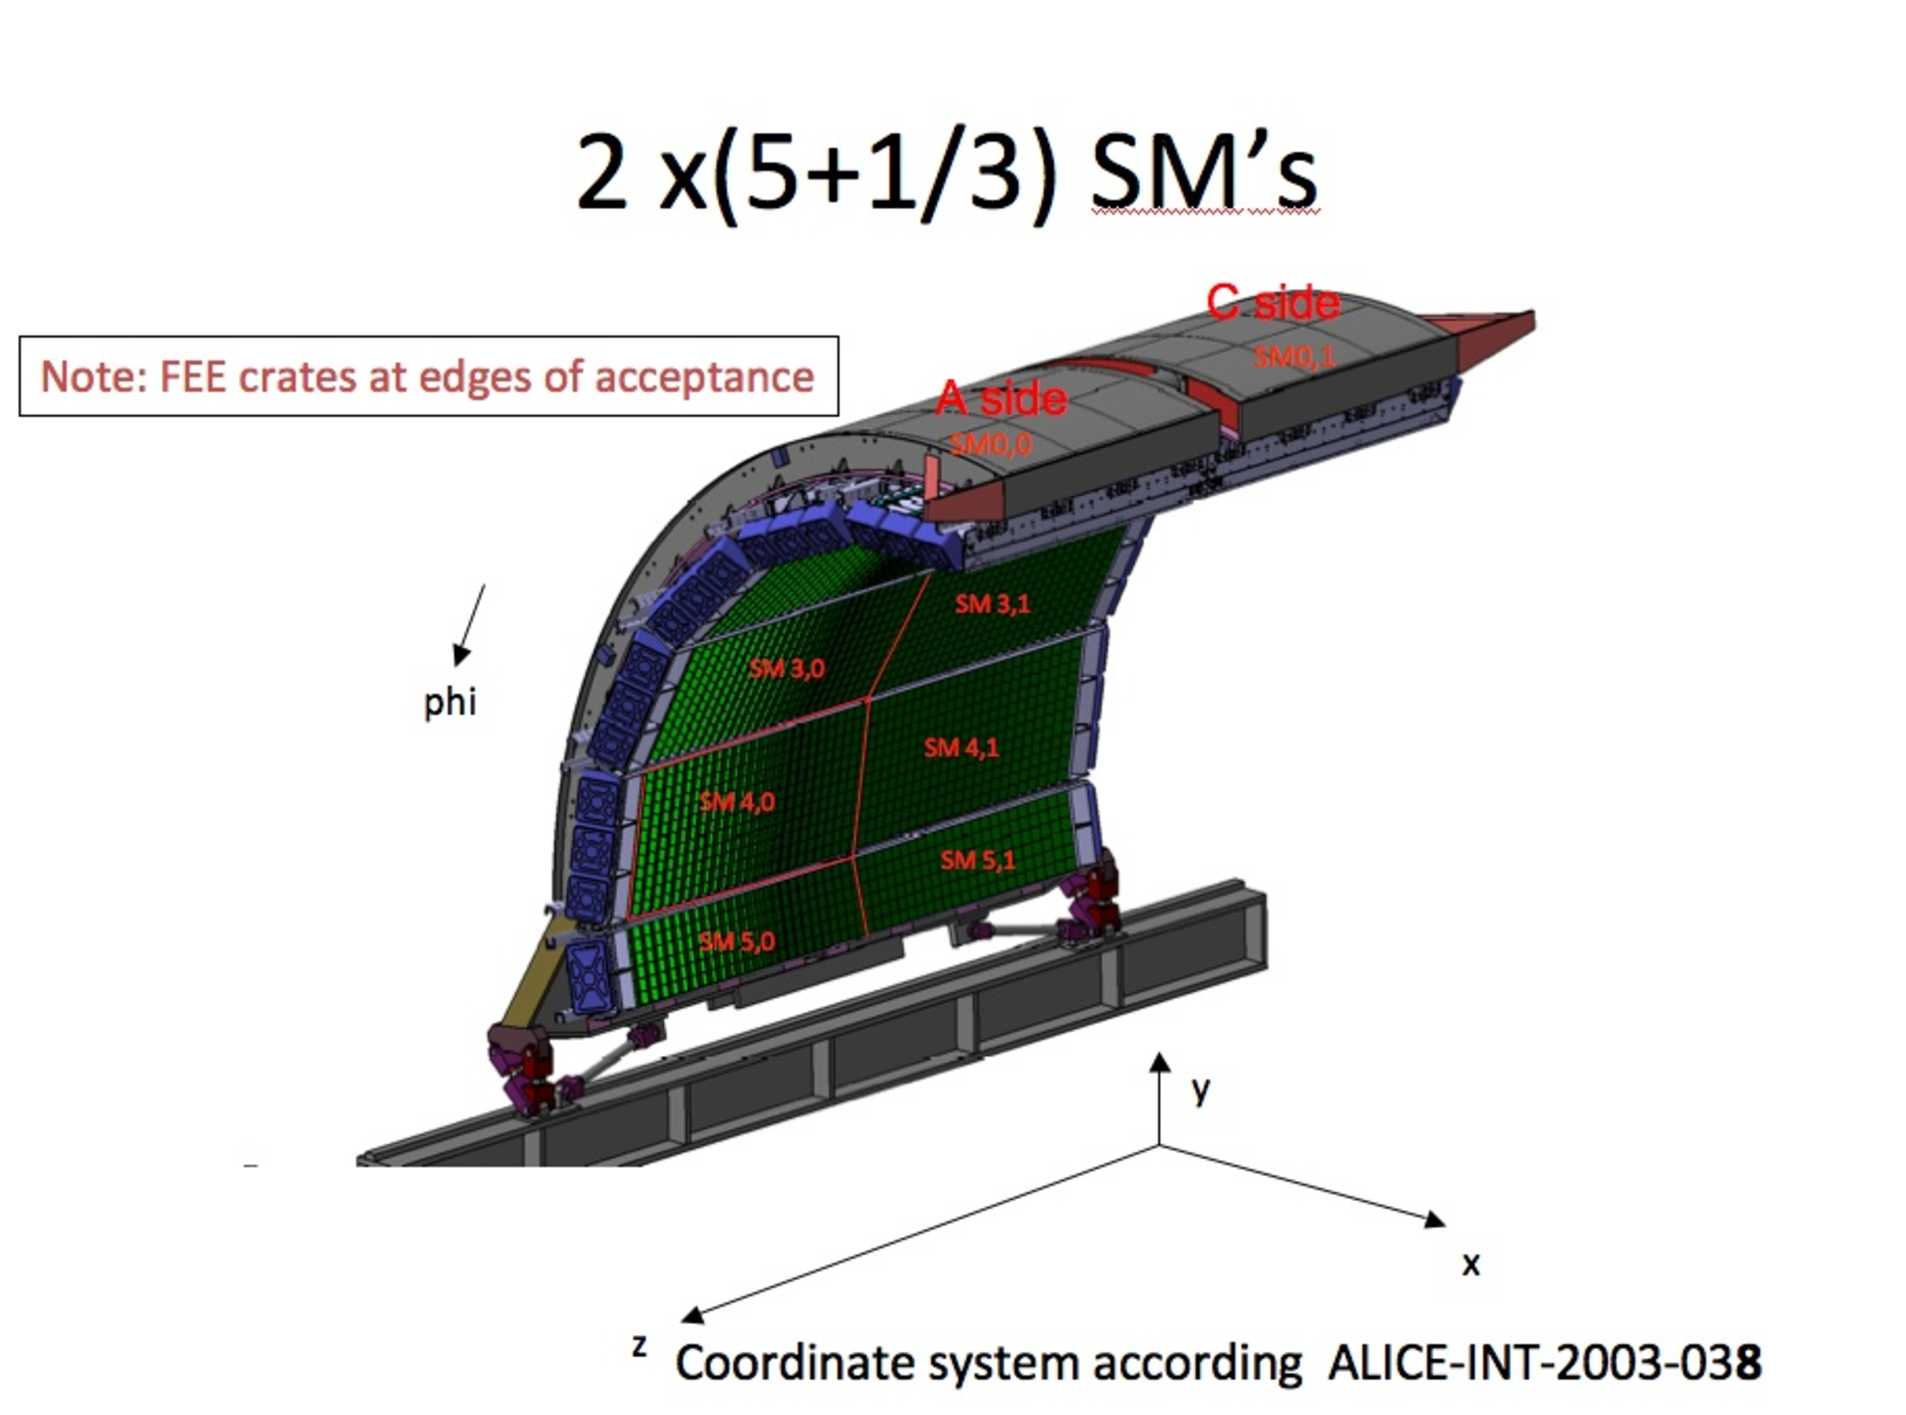
\includegraphics[width=1.0\textwidth]{figures/EMCALMap0_0.pdf}
\end{center}
\caption{\label{fig:Map1}Position of the super modules}
\end{figure}

\begin{figure}[ht]
\begin{center}
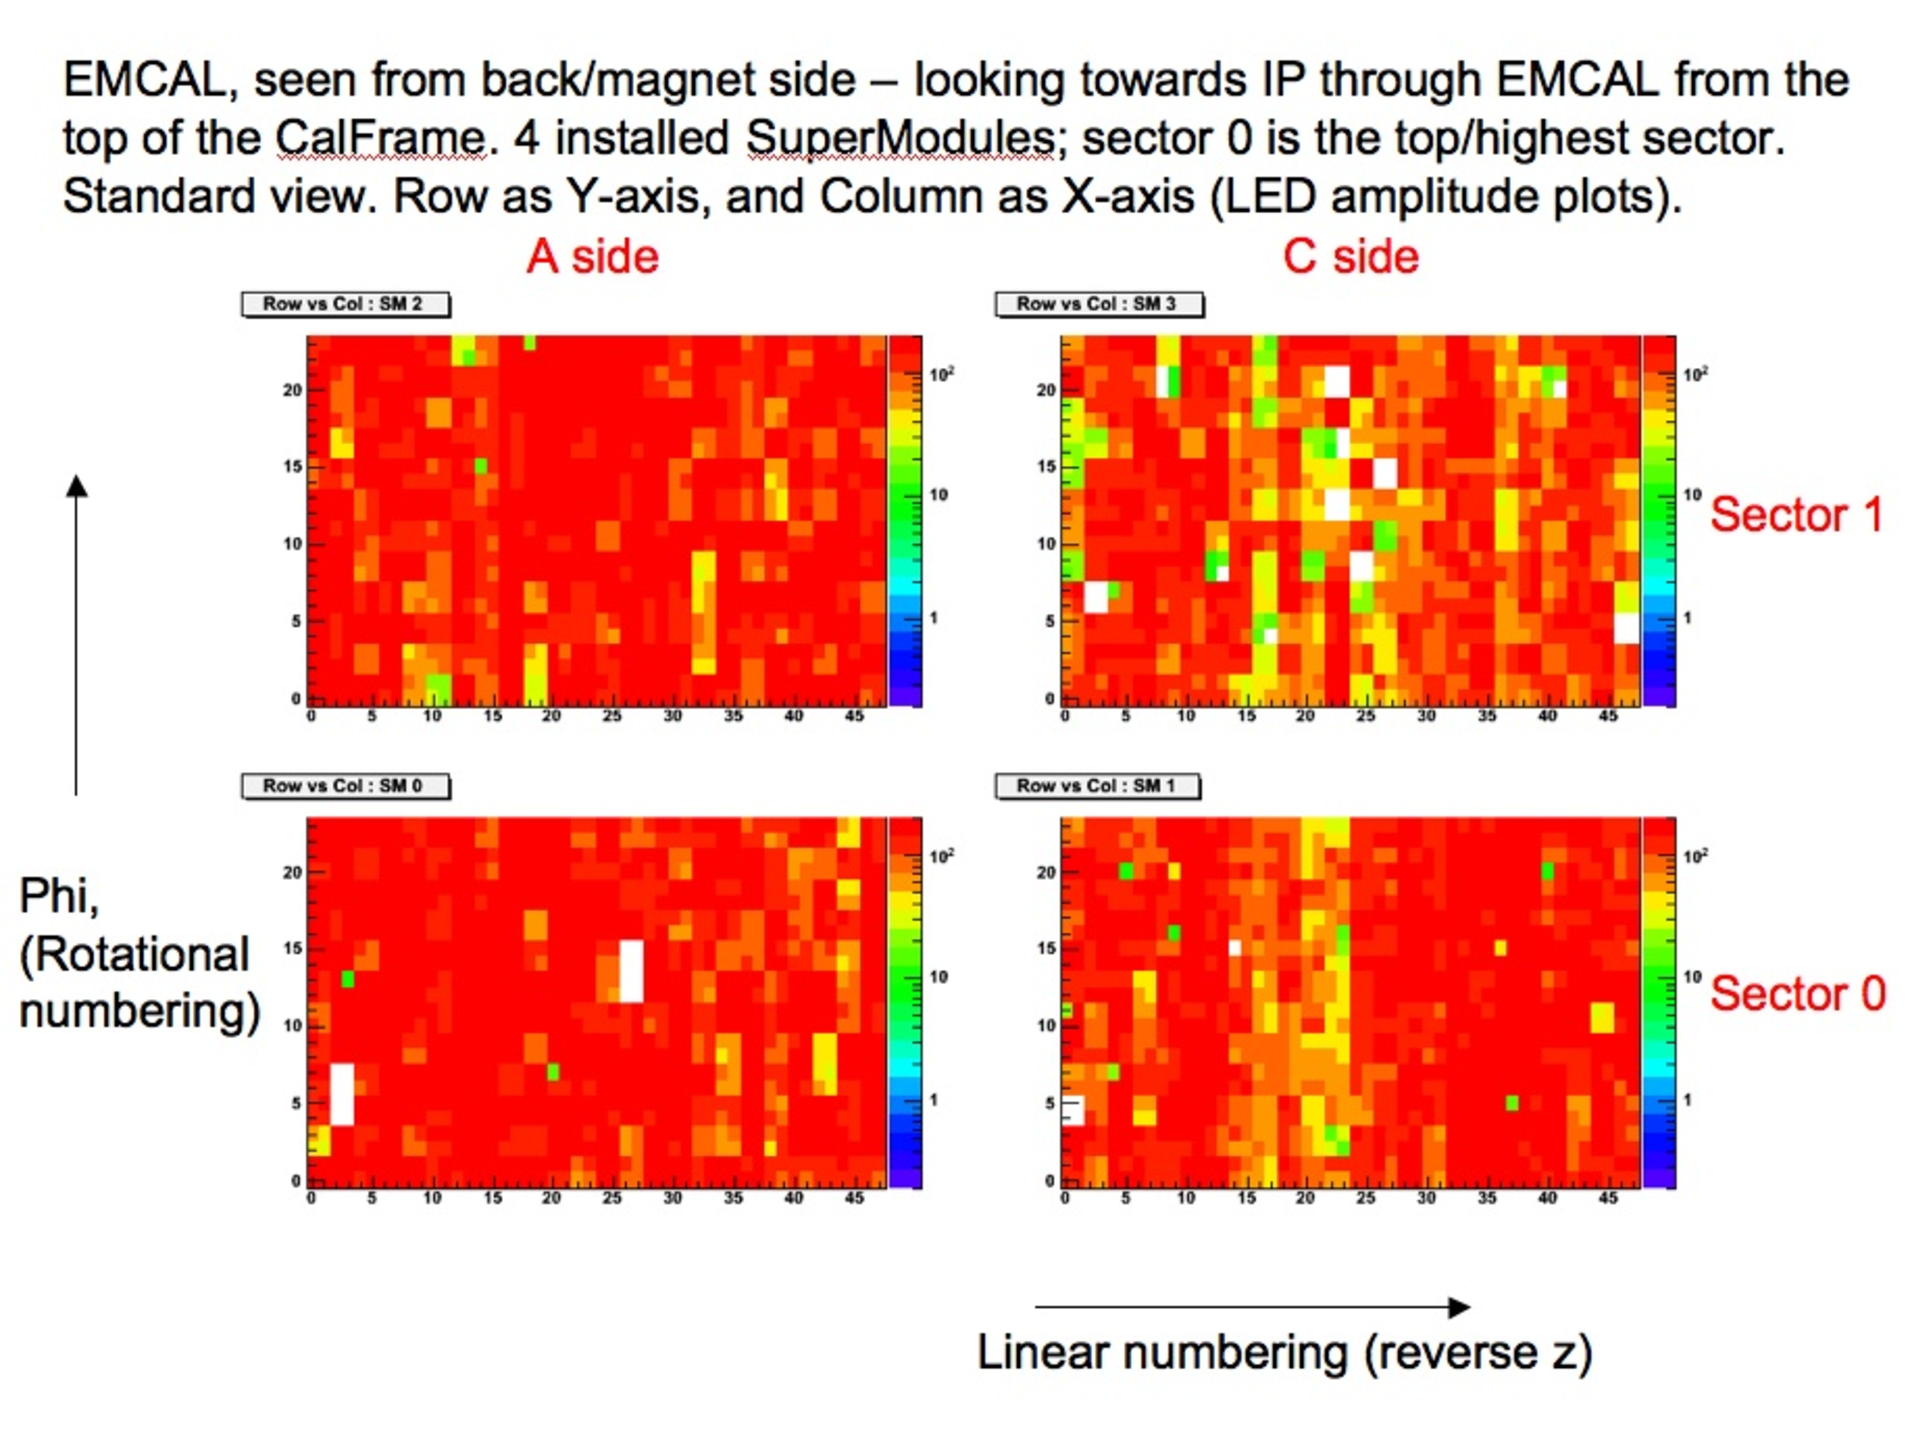
\includegraphics[width=1.0\textwidth]{figures/EMCALMap1.pdf}
\end{center}
\caption{\label{fig:Map0}EMCal seen from the magnet side with 4 SMs.}
\end{figure}


\begin{figure}[ht]
\begin{center}
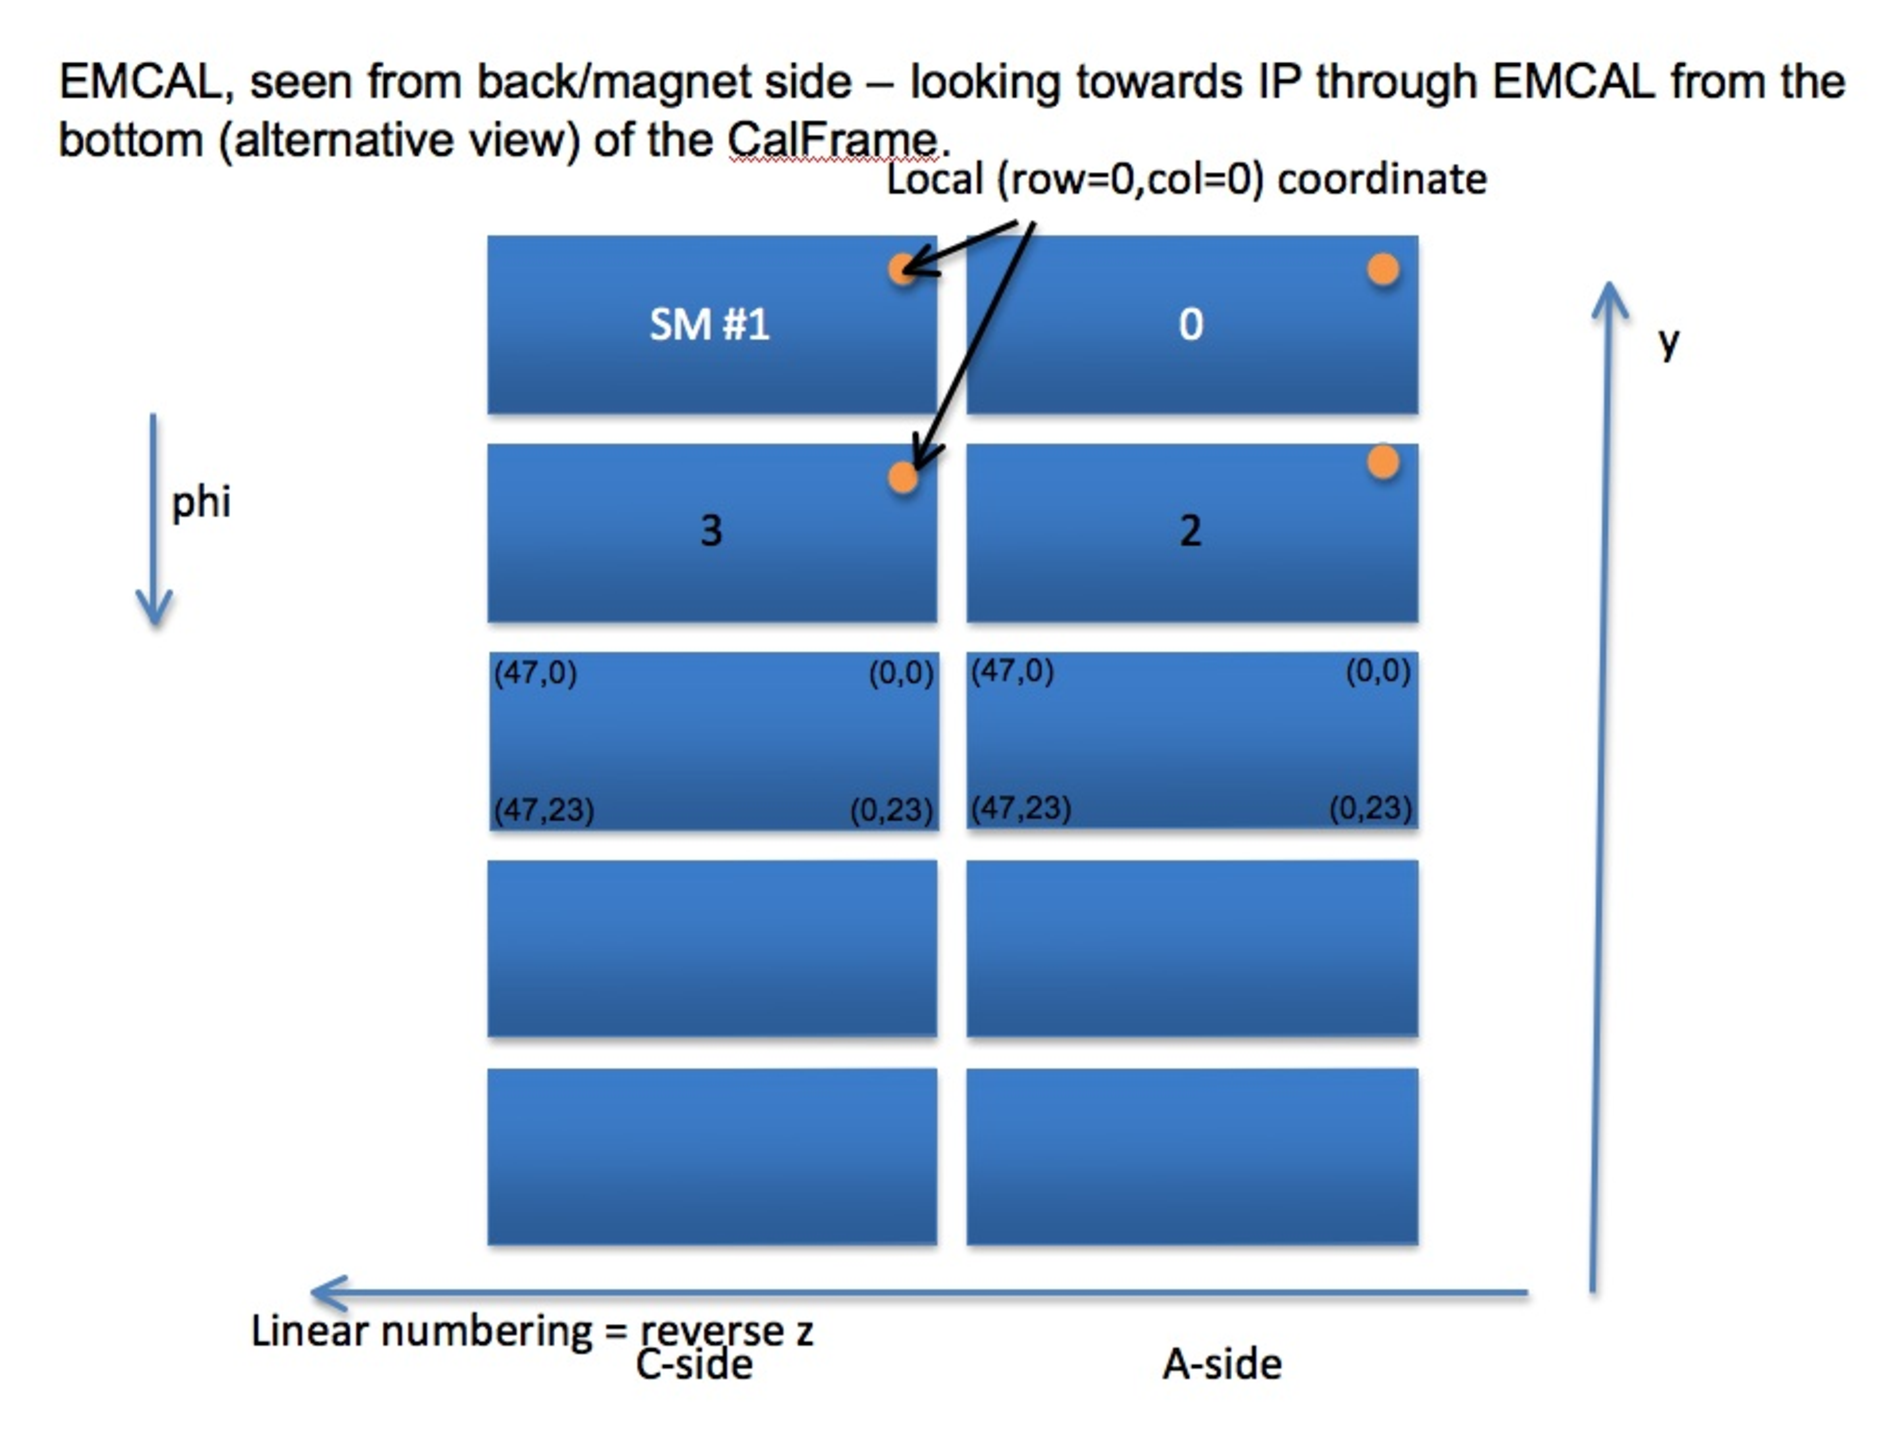
\includegraphics[width=1.0\textwidth]{figures/EMCALMap2.pdf}
\end{center}
\caption{\label{fig:Map2}EMCal geometrical numbering.}
\end{figure}


\subsection{Tower index transformation methods}
\subsubsection{Absolute tower ID to Row/Column index}

Each EMCAL supermodule is composed of 24x48 towers (phi,eta), grouped in 4x4 modules. Each tower (even each module) has a unique number assigned, called in the code "absolute ID" number (absId). This number can be transformed into a row (phi direction) or column (eta direction) index. The procedure to go from the absId to the (row, col) formulation or viceversa is as follow:

\begin{itemize}
\item From absId to col-row: 

\begin{DDbox}{\linewidth}
\begin{lstlisting}
Int_t nSupMod, nModule, nIphi, nIeta, iphi, ieta;
//Check if this absId exists
if(!CheckAbsCellId(absId)) return kFALSE;
// Get from the absId the super module number, the module number and the eta-phi index (0 or 1) in the module
GetCellIndex(absId, nSupMod, nModule, nIphi, nIeta);
// Get from the  the super module number, the module number and the eta-phi index (0 or 1) in the module the tower row (iphi) and column (ieta) 
GetCellPhiEtaIndexInSModule(nSupMod,nModule,nIphi,nIeta, iphi, ieta); 
\end{lstlisting}
\end{DDbox}

\item From col-row to absId, following the same notation as above: 

\begin{DDbox}{\linewidth}
\begin{lstlisting}

absid = GetAbsCellIdFromCellIndexes(nSupMode, iphi, ieta);
\end{lstlisting}
\end{DDbox}

or

\begin{DDbox}{\linewidth}
\begin{lstlisting}

absid = GetAbsCellId(nSupMod, nModule, nIphi, nIeta);
\end{lstlisting}
\end{DDbox}

\item Other interesting method is

\begin{DDbox}{\linewidth}
\begin{lstlisting}

Int_t   GetSuperModuleNumber(Int_t absId)  
\end{lstlisting}
\end{DDbox}
\end{itemize}

\subsection{Tower index to local / global reference system position}
\subsubsection{Local coordinates}

To correlate the tower index and its position in local coordinates, the following methods are available:

\begin{DDbox}{\linewidth}
\begin{lstlisting}
  Bool_t  AliEMCALGeoUtils::RelPosCellInSModule(Int_t absId, Double_t &xr, Double_t &yr, Double_t &zr) const;

  Bool_t  AliEMCALGeoUtils::RelPosCellInSModule(Int_t absId, Double_t loc[3]) const;

  Bool_t  AliEMCALGeoUtils::RelPosCellInSModule(Int_t absId, TVector3 &vloc) const;
\end{lstlisting}
\end{DDbox}

To which the input is the absId and the output are the coordinates of the center of towers in the local coordinates of the Super Module. This method gets the column and row index of the cell from the absId, independently of the Super Module (like above), and gets the center of the cell from 3 arrays (x,y,z) filled with such quantities. Such central positions are calculated during the initialization of the geometry, where the arrys are filled, in the method :

\begin{DDbox}{\linewidth}
\begin{lstlisting}

  AliEMCALGeoUtils::CreateListOfTrd1Modules()
\end{lstlisting}
\end{DDbox}

{\color{red}<<<<<Someone else should explain how it works>>>>>}

 

In case we calculate the cluster position, things are a bit different.

 

{\color{red}<<<<< This explanation should go to the clusterization section>>>>}

 

This is done in 

\begin{DDbox}{\linewidth}
\begin{lstlisting}
void AliEMCALRecPoint::EvalLocalPosition()
\end{lstlisting}
\end{DDbox}

First we calculate the cell position with the  method 

\begin{DDbox}{\linewidth}
\begin{lstlisting}
AliEMCALGeometry::RelPosCellInSModule(Int_t absId, Int_t maxAbsId, Double_t tmax, Double_t &xr, Double_t &yr, Double_t &zr)
\end{lstlisting}
\end{DDbox}

The calculation of the cell position done here is different in the "x-z" but the same in "y". 

 

{\color{red}<<<<< <<<<<Someone else should explain how it works>>>>>}

 
 

In this particular case the position calculation per tower depends on the position of the maximum cell, and the sum of the energy of the cells of the cluster. The maximum depth (tmax) is calculated with the method

\begin{DDbox}{\linewidth}
\begin{lstlisting}
  Double\t AliEMCALRecPoint::TmaxInCm(const Double_t e){

      //e: energy sum of cells

static Double_t ca = 4.82;// shower max parameter - first guess; ca=TMath::Log(1000./8.07)

      static Double_t x0 = 1.23; // radiation lenght (cm)

      static Double_t tmax = 0.; // position of electromagnetic shower max in cm

      tmax = TMath::Log(e) + ca+0.5;

      tmax *= x0; // convert to cm

  }
\end{lstlisting}
\end{DDbox}

After the cells position of the cluster is accessed, the position of the cluster is calculated averaging the cell positions with a logarithmic weight:

\begin{DDbox}{\linewidth}
\begin{lstlisting}
  w(cell i) = TMath::Max( 0., logWeight + TMath::Log( energy[cell i] / summed_cluster_cell_energy ));
\end{lstlisting}
\end{DDbox}

where the logWeight was chosen to be 4.5 (this value was taken from PHOS, never optimized as far as I know)

So in the end the position,  is 

\begin{DDbox}{\linewidth}
\begin{lstlisting}
f = Sum(f(i) * w(i))/Sum(w(i))
\end{lstlisting}
\end{DDbox}

where f=x,y,z.

 

 \subsubsection{Global coordinates}
 

To transform from local to global we have the methods

\begin{DDbox}{\linewidth}
\begin{lstlisting}

  void GetGlobal(const Double_t *loc, Double_t *glob, int ind) const;

  void GetGlobal(const TVector3 &vloc, TVector3 &vglob, int ind) const;

  void GetGlobal(Int_t absId, Double_t glob[3]) const;

  void GetGlobal(Int_t absId, TVector3 &vglob) const;
\end{lstlisting}
\end{DDbox}

 

 These methods take the local coordinates and transform them into global coordinates using the transformation matrix of the Super Module.

\begin{DDbox}{\linewidth}
\begin{lstlisting}
 

TGeoHMatrix* m = GetMatrixForSuperModule(nSupMod);

if(m) m->LocalToMaster(loc, glob);

\end{lstlisting}
\end{DDbox}
 

 GetGlobal is called in the following useful methods in the geometry class:

 
\begin{itemize}
\item Return the eta and phi angular position of the cell from the AbsId

\begin{DDbox}{\linewidth}
\begin{lstlisting}
void    EtaPhiFromIndex(Int_t absId, Double_t &eta, Double_t &phi) const;
void    EtaPhiFromIndex(Int_t absId, Float_t &eta, Float_t &phi) const;
\end{lstlisting}
\end{DDbox}
\item Print information of the cells. For "pri>0" returns more information. "tit" has not much use, this value is printed.

\begin{DDbox}{\linewidth}
\begin{lstlisting}
void PrintCellIndexes(Int_t absId, int pri, const char *tit)
\end{lstlisting}
\end{DDbox}
\end{itemize} 

\subsection{Geometry Alignment}
AliRoot contains a frame for the correction of the misplacement of geometry objects with respect to the ideal positions which are kept in the STEER/ directory of the following classes:

\begin{DDbox}{\linewidth}
\begin{lstlisting}
AliAlignObj  
AliAlignObjMatrix  
AliAlignObjParams  
AliAlignmentTracks
\end{lstlisting}
\end{DDbox}

The class AliEMCALSurvey creates the corrections to the alignable objects.  The class AliEMCALSurvey was established to take the survey parameters from OCDB, calculate the shift in position of the center of the end faces of the supermodules from the nominal position, and convert this to a transformation matrix for each supermodule which is applied to correct the global position of the supermodules.  All calculations of global positions would then use these corrected supermodule positions to determine their locations within the ALICE global coordinate system. 
